\documentclass[../sotsu.tex]{subfiles}

\graphicspath{{../fig/}}

\begin{document}

\section{ベクトル空間}

量子力学において,系の状態は「ベクトル」を用いてであらわされる.
しかし,通常の\ruby{数}{すう}ベクトルでは量子力学的状態をあらわせないことがわかる(ここでどこかを引用する).
そこで,数ベクトルの概念を一般化・抽象化する必要がある.
この章ではベクトルの性質を抽象化し,ベクトル空間について定義する.

\subsection*{序:3次元ユークリッド空間$\symbb{R}^3$の性質}
\addcontentsline{toc}{subsection}{\numberline{序}3次元ユークリッド空間\texorpdfstring{$\symbb{R}^3$}{ℝ³}の性質}

この節では,数ベクトルの性質を確かめる.

$n$個の数字\footnote{ここでは実数または複素数のこと.}を縦に並べたものを「$n$-\ruby{次}{じ}の\ruby{列}{れつ}ベクトル」と呼び,
横に並べたものを「$n$-次の\ruby{行}{ぎょう}ベクトル」と呼ぶ\cite{miyake-lin-2008}.
列ベクトルのことを「\ruby{縦}{たて}ベクトル」,行ベクトルを「\ruby{横}{よこ}ベクトル」ということもある.

たとえば\cref{eq:Euclidean-vector-example}の$\symbf{x}$は3次の列ベクトル,
$\symbf{y}$は3次の行ベクトルである.
\begin{align}
    \label{eq:complex-Euclidean-vector-example}
    \symbf{x} = 
    \begin{pmatrix}
        a  \\  b  \\  c
    \end{pmatrix}
    , \qquad
    \symbf{y} = 
    \begin{pmatrix}
        a  &  b  &  c
    \end{pmatrix}
    \qquad 
    \text{where $a, b, c \in \symbb{C}$}
\end{align}
ここで,$a, b, c$はそれぞれある複素数である\footnote{$\symbb{C}$は複素数全体の集合.\cref{eq:number-sets}を参照}.
$a, b, c$のことをそれぞれ,ベクトルの\word{成分}[せい|ぶん]という.

列ベクトルと行ベクトルは,「\word{転置}[てん|ち](transpose)」という操作によって移り変わる.
つまり,
\begin{equation*}
    \tp{\begin{pmatrix}
        a  \\  b  \\  c
    \end{pmatrix}}
    =
    \begin{pmatrix}
        a  &  b  &  c
    \end{pmatrix},
    \quad
    \tp{\begin{pmatrix}
        a  &  b  &  c
    \end{pmatrix}}
    =
    \begin{pmatrix}
        a  \\  b  \\  c
    \end{pmatrix}
\end{equation*}
である.
列ベクトルを,転置を用いて$\tp{(a \quad b \quad c)}$と表記することもある.

ベクトル$\tp{(a, b, c)}$は,ある点から$x$-軸方向へ$a$,$y$-軸方向へ$b$,$z$-軸方向へ$c$だけ動いた点を結ぶ矢印として考えることができる.

ベクトル同士の「\ruby{和}{わ}」(足し算)を
\begin{equation*}
    \begin{pmatrix}
        a  \\  b  \\  c
    \end{pmatrix}
    \vecplus
    \begin{pmatrix}
        a' \\ b' \\ c'
    \end{pmatrix}
    =
    \begin{pmatrix}
        a + a'  \\  b + b'  \\  c + c'
    \end{pmatrix}
\end{equation*}
のように,各成分の和として定義する.
ベクトルの和は,2つの矢印をつなげた見たときの矢印に相当する(\cref{fig:vector-sum}).

また,ベクトルの「\word{スカラー倍}」を、
\begin{equation*}
    \lambda \scaprod 
    \begin{pmatrix}
        a  \\  b  \\  c
    \end{pmatrix}
    =
    \begin{pmatrix}
        \lambda a  \\  \lambda b  \\  \lambda c
    \end{pmatrix}
\end{equation*}
で定義する。
ベクトルのスカラー倍は、向きを保ったまま長さを$\lambda$倍した矢印に対応する(\cref{fig:vector-scalar-p})。

\begin{figure}[tbp]
    \centering
    \begin{subcaptionblock}{0.4\linewidth}
        \centering
        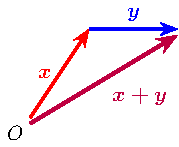
\includegraphics[width=0.9\linewidth]{vector_sum.pdf}
        \caption{ベクトルの和}
        \label{fig:vector-sum}
    \end{subcaptionblock}
    \begin{subcaptionblock}{0.4\linewidth}
        \centering
        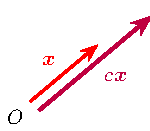
\includegraphics[width=0.9\linewidth]{vector_scalar_p.pdf}
        \caption{ベクトルのスカラー倍}
        \label{fig:vector-scalar-p}
    \end{subcaptionblock}
    \caption{ベクトルの演算}
\end{figure}

このように定義されたベクトルの和とスカラー倍についての性質を抽出したのが\cref{dfn:vector-space}である。



\subsection{ベクトル空間の定義}

\begin{definition}[ベクトル空間]
    \label{dfn:vector-space}
    $V$を集合,$(\symbb{K}, +, \dotprod)$を体\refdfn{dfn:field}とする.
    $V$上の\word{和}$\vecplus\colon V \times V \to V$,\word{スカラー倍}$\scaprod \colon \symbb{K} \times V \to V$が定義され,
    以下が満たされるとき,$(V, \vecplus, \scaprod)$を($\symbb{K}$上の)\word{ベクトル空間}(vector space)あるいは\word{線形空間}[せん|けい|くう|かん](linear space)という.
    このとき$V$の元を\word{ベクトル}(vector),$\symbb{K}$の元を\word{スカラー}(scalar)という.
    \begin{enumerate}
        \item \label{vector:sum-associative} 任意の$\symbf{u}, \symbf{v}, \symbf{w} \in V$に対して,$(\symbf{u} \vecplus \symbf{v}) \vecplus \symbf{w} = \symbf{u} \vecplus (\symbf{v} \vecplus \symbf{w})$である.
        \item \label{vector:sum-zero} ある$\symbf{0} \in V$が存在し,任意の$\symbf{v} \in V$に対して,$\symbf{v} \vecplus \symbf{0} = \symbf{0} \vecplus \symbf{v} = \symbf{v}$である.
        \item \label{vector:sum-opposite} 任意の$\symbf{v} \in V$に対して,ある$-\symbf{v}$が存在して,$\symbf{v} \vecplus (-\symbf{v}) = (-\symbf{v}) \vecplus \symbf{v} = \symbf{0}$である.
        \item \label{vector:sum-commutative} 任意の$\symbf{u}, \symbf{v} \in V$に対して,$\symbf{u} \vecplus \symbf{v} = \symbf{v} \vecplus \symbf{u}$である.
        \item \label{vector:scalar-distributive} 任意の$\symbf{u}, \symbf{v} \in V$および任意の$c \in \symbb{K}$に対して,$c \scaprod (\symbf{u} \vecplus \symbf{v}) = (c \scaprod \symbf{u}) \vecplus (c \scaprod \symbf{v})$である.
        \item \label{vector:scalar-sum} 任意の$\symbf{v} \in V$および任意の$a, b$に対して,$(a + b) \scaprod \symbf{v} = (a \scaprod \symbf{v}) \vecplus (b \scaprod \symbf{v})$である.
        \item \label{vector:scalar-prod} 任意の$\symbf{v} \in V$および任意の$a, b$に対して,$(a \dotprod b) \scaprod \symbf{v} = a \scaprod (b \scaprod \symbf{v})$である.
        \item \label{vector:scalar-identity} 任意の$\symbf{v} \in V$に対して,$1 \scaprod \symbf{v} = \symbf{v}$である.
    \end{enumerate}
    ベクトル空間$(V, \vecplus, \scaprod)$のことを単に$V$と書くこともある.
\end{definition}

\begin{corollary}
    ベクトル空間$V$は以下を満たす.
    \begin{itemize}
        \item 零ベクトルについて,
        \begin{enumerate}
            \item $\symbf{0}$は一意に定まる.
        \end{enumerate}
        \item 任意の$\symbf{v} \in V$に対し,
        \begin{enumerate}[resume]
            \item $-\symbf{v}$は一意に定まる.
            \item $ 0 \scaprod \symbf{v} = \symbf{0} $である.
            \item $ (-1) \scaprod \symbf{v} = -\symbf{v} $である.
        \end{enumerate}
    \end{itemize}
\end{corollary}

\begin{proof}
    \begin{enumerate}
        \item 零ベクトル$\symbf{0}, \symbf{0}'$をとると,$\symbf{0} = \symbf{0} \vecplus \symbf{0}' = \symbf{0}'$.
        \item $\symbf{v}$の逆元として$\symbf{u}, \symbf{u}'$をとると,
            $\symbf{u}  =  \symbf{u} \vecplus (\symbf{v} \vecplus \symbf{u}')  =  (\symbf{u} \vecplus \symbf{v}) \vecplus \symbf{u}'  =  \symbf{u}'$.
        \item $ 0 \scaprod \symbf{v} = (0 + 0) \scaprod \symbf{v} = 0 \scaprod \symbf{v} \vecplus 0 \scaprod \symbf{v} $より従う.
        \item $ \symbf{v} \vecplus (-1) \scaprod \symbf{v} = 1 \scaprod \symbf{v} \vecplus (-1) \scaprod \symbf{v} = (1 + (-1)) \scaprod \symbf{v} = 0 \scaprod \symbf{v} = \symbf{0} $より従う.
    \end{enumerate}
\end{proof}

$\symbf{v} \vecplus (-\symbf{u}) \eqcolon \symbf{v} \vecminus \symbf{u}$とかくことが多い.


\begin{example}
    実ユークリッド空間$\symbb{R}^n$は,適切な和とスカラー倍の下で$\symbb{R}$上のベクトル空間になる.
    また,複素ユークリッド空間$\symbb{C}^n$は,$\symbb{R}$上のベクトル空間であり,また$\symbb{C}$上のベクトル空間でもある.
\end{example}


\subsection{部分ベクトル空間}

\begin{definition}[部分ベクトル空間]
    \label{dfn:vector-subspace}
    $V$をベクトル空間,$W \subset V$とする.
    $W$が$V$の和とスカラー倍に対してベクトル空間になるとき,$W$は$U$の\word{部分ベクトル空間}(vector subspace)あるいは単に\word{部分空間}(subspace)であるという.
\end{definition}

部分空間と部分集合を取り違えないように注意が必要である。
部分集合のうちベクトル空間になるものが部分空間(部分ベクトル空間)である。

\begin{theorem}
    \label{thm:vector-subspace-iff}
    $V$をベクトル空間とする.$U \subset V$が以下の条件を満たす場合,$U$は$V$の部分ベクトル空間になる.
    \begin{enumerate}
        \item \label{vector-subspace:sum-closed} 任意の$\symbf{u}, \symbf{v} \in U$に対し,$\symbf{u} \vecplus \symbf{v} \in U$である($U$は和で閉じている).
        \item \label{vector-subspace:scalar-closed} 任意の$\symbf{v} \in U$および任意の$c \in \symbb{K}$に対し,$c \scaprod \symbf{v} \in U$である($U$はスカラー倍で閉じている).
        \item \label{vector-subspace:zero} $\symbf{0} \in U$である.
    \end{enumerate}
    \cref{vector-subspace:zero}は\cref{vector-subspace:scalar-closed}で$c=0$とすれば自動的に満たされるように見える.
    この条件をわざわざ加えるのは,$U \neq \emptyset$であることを保証するためである.
\end{theorem}


\begin{proposition}
    \label{thm:intersection-of-vector-space}
    $V$をベクトル空間、$W_1, W_2 \subset V$を部分ベクトル空間とする。
    このとき共通部分\refdfn{dfn:intersection-of-set}$W_1 \cap W_2$は$V$の部分ベクトル空間である。
\end{proposition}

\begin{proof}
    \cref{thm:vector-subspace-iff}を確かめればよい。
\end{proof}


\begin{definition}[和空間]
    \label{dfn:sum-of-vector-space}
    $V$をベクトル空間、$W_1, W_2 \subset V$を部分ベクトル空間とする。
    \begin{equation}
        W_1 + W_2 \coloneq \Set{  \symbf{v}_1 \vecplus \symbf{v}_2  \given  \symbf{v}_1 \in W_1, \  \symbf{v}_2 \in W_2  }
    \end{equation}
    は$V$の部分ベクトル空間である。
\end{definition}
なお、和空間$W_1 + W_2$と和集合\refdfn{dfn:union-of-set}$W_1 \cup W_2$は異なる概念である。
一般に$W_1 \cup W_2$は部分ベクトル空間にならない。

\begin{definition}[直和空間]
    \label{dfn:direct-sum-of-vector-space}
    和空間$W_1 + W_2$で、特に$W_1 \cap W_2 = \{ \symbf{0} \}$であるとき、
    \word{直和}[ちょく|わ][ちよくわ](direct sum)といい、
    $W_1 \oplus W_2$とかく。
\end{definition}



\subsection{ベクトルの一次独立・一次従属}

\begin{definition}[ベクトルの線形結合]
    \label{dfn:linear-combination}
    $V$を$\symbb{K}$上のベクトル空間,$\symbf{v}_1, \symbf{v}_2, \dotsc \in V$をベクトル,$c_1, c_2, \dotsc \in \symbb{K}$を有限個を除いてゼロであるスカラーとする.
    このとき,ベクトル$\symbf{v} = c_1 \symbf{v}_1 \vecplus c_2 \symbf{v}_2 \vecplus \dotsb$のことを,
    ベクトル$\symbf{v}_1, \symbf{v}_2, \dotsc$の\word{線形結合}[せん|けい|けつ|ごう](linear combination)あるいは\word{一次結合}[いち|じ|けつ|ごう]という.
\end{definition}

\cref{dfn:linear-combination}において,
$c_i$が有限個を除きゼロである,つまり$c_1 \symbf{v}_1 \vecplus c_2 \symbf{v}_2 \vecplus \dotsb$が有限和であるという条件は重要である.
一般に,無限和では$c_1 \symbf{v}_1 \vecplus c_2 \symbf{v}_2 \vecplus \dotsb \in V$とは限らない.
たとえば,実関数$e^x$は多項式ベクトル空間の元$1, x, x^2, x^3, \dotsc \in \symbb{R}[x]$を使って
\begin{equation*}
    e^x = 1 + x + \frac{1}{2!} x^2 + \frac{1}{3!} x^3 + \dotsb
\end{equation*}
と書けるが,明らかに$e^x \notin \symbb{R}[x]$である.


\begin{definition}[ベクトル空間の生成系]
    \label{dfn:spanning-set}
    $V$を$\symbb{K}$上のベクトル空間,$W \subset V$を部分ベクトル空間とする.
    ベクトルの組$\symbf{v}_1, \symbf{v}_2, \dotsc \in V$が$W$を\word{生成する}(generate)あるいは\word{張る}(span)とは,
    $\symbf{v}_1, \symbf{v}_2, \dotsc \in V$から有限個のベクトル$\symbf{u}_1, \dots, \symbf{u}_n$を任意にとったときの線形結合の全体が$W$に一致する,すなわち
    \begin{equation*}
        W = \Set{ c_1 \symbf{v}_1 \vecplus c_2 \symbf{v}_2 \vecplus \dotsb \in V  \given  c_1, c_2, \dotsc \in \symbb{K}, \  \text{$c_i$は有限個を除きゼロ}} \subset V
    \end{equation*}
    であることをいう.
    また,$\symbf{v}_1, \symbf{v}_2, \dotsc \in V$が生成する部分ベクトル空間を
    \begin{equation}
        \label{eq:spanning-set-notation}
        W = \spanning{\symbf{v}_1, \symbf{v}_2, \dotsc}
    \end{equation}
    とかく.
\end{definition}

\begin{definition}[一次独立と一次従属]
    \label{dfn:linearly-independent}
    $V$を$\symbb{K}$上のベクトル空間とする.
    ベクトルの組$\symbf{v}_1, \symbf{v}_2, \dotsc \in V$が\word{一次独立}[いち|じ|どく|りつ](linearly independent)あるいは\word{線形独立}であるとは,
    有限個を除き$0$である$c_1, c_2, \dotsc \in \symbb{K}$に対し,
    \begin{equation*}
        c_1 \symbf{v}_1 \vecplus c_2 \symbf{v}_2 \vecplus \dotsb = \symbf{0}
        \iff
        c_1 = c_2 = \dots = 0
    \end{equation*}
    であることをいう.
    ベクトルの組$\symbf{v}_1, \symbf{v}_2, \dotsc \in V$が一次独立でないとき,\word{一次従属}[いち|じ|じゅう|ぞく](linearly dependent)あるいは\word{線形従属}という.
\end{definition}


\subsection{ベクトル空間の基底と次元}

\begin{definition}[基底]
    \label{dfn:basis}
    $V$を$\symbb{K}$上のベクトル空間とする.
    ベクトルの組$ \{ \symbf{v}_1, \symbf{v}_2, \dotsc \} \subset V$は,以下を満たすとき,\word{基底}[き|てい](basis)という.
    \begin{enumerate}
        \item \label{base:linearly-independent} $\symbf{v}_1, \symbf{v}_2, \dotsc$は一次独立である.
        \item \label{base:spans-V} $\symbf{v}_1, \symbf{v}_2, \dotsc$は$V$を生成する.
            すなわち,任意の$\symbf{v} \in V$に対して,有限個を除き$0$の,ある$c_1, c_2, \dotsc \in \symbb{K}$が存在し,$\symbf{v} = c_1 \symbf{v}_1 + c_2 \symbf{v}_2 + \dotsb$とかける.
    \end{enumerate}
\end{definition}

\begin{example}
    $ \{ (1, 0, 0), \ (0, 1, 0), \ (0, 0, 1) \} $は$\symbb{R}^3$の基底である.
    また,$ \{ (1, 1, 0), \ (1, -1, 0), \ (0, 0, 1) \} $も$\symbb{R}^3$の基底である.
\end{example}

例でみたように,一般にベクトル空間$V$が与えられたとき,その基底の取り方は一意ではない.
しかし,基底を構成するベクトルの数は,基底の取り方によらない.
\begin{proof}
    なんかかく
\end{proof}

\begin{definition}[次元]
    \label{dfn:dimension}
    $V$をベクトル空間とする.
    $V$の基底を構成するベクトルの数を\word{次元}[じ|げん](dimension)といい,$\dim V$とかく.
\end{definition}

\begin{example}
    多項式ベクトル空間$\symbb{R}[x]$について,$\{ 1, x, x^2, \dotsc \}$は一次独立であり,さらに基底をなす.
    このように,ベクトル空間$V$の基底を構成するベクトルの数は無限個であるとき,$V$は\word{無限次元}(infinite dimensional)であるという.
\end{example}

\begin{example}
    複素数全体の集合$\symbb{C}$は、
    $\symbb{C}$上のベクトル空間と考えると$\dim_{\symbb{C}} = 1$(基底$1$)、
    $\symbb{R}$上のベクトル空間と考えると$\dim_{\symbb{R}} = 2$(基底$1, \iu$)である。
\end{example}


\begin{corollary}[基底によるベクトルの展開]
    \label{thm:coordinates-by-basis}
    $V$をベクトル空間とする.
    任意の$\symbf{v} \in V$は,$V$の基底$ \{ \symbf{u}_i \} $のうち有限個を用いて$\symbf{v} = c_1 \symbf{v}_1 \vecplus \dots \vecplus c_n \symbf{v}_n$とかける.
    このとき,スカラーの組$c_1, \dots, c_n \in \symbb{K}$は一意に定まる.
\end{corollary}

\begin{proof}
    前半は基底の定義\refdfn{dfn:basis}より明らかなので,一意性を示す.
    $\symbf{v} = a_1 \symbf{u}_1 \vecplus \dots \vecplus a_n \symbf{u}_n = b_1 \symbf{u}_1 \vecplus \dots \vecplus b_n \symbf{u}_n$と2通りにかけたとすると,
    \begin{equation*}
        (a_1 \! - b_1) \symbf{u}_1 \vecplus \dots \vecplus (a_n \! - b_n) \symbf{u}_n = \symbf{0}
    \end{equation*}
    がいえるが,基底は一次独立なので$a_1 \! - b_1 = \dots = a_n \! - b_1 = 0$である.
\end{proof}



\subsubsection{任意のベクトル空間に基底が存在する}

ここまでは,ベクトル空間に基底が存在すると仮定したうえで議論してきた.
実は,任意のベクトル空間について,基底が存在することを示すことができる.

証明にはツォルンの補題を用いる。


\end{document}